% -------------------------------------------------------------------------------------- %

\section{Numerical Examples}

We demonstrate the error in observables for multiple initial conditions. We show that 
the proposed methods indeed satisfy conservation laws as stated in theorem 
\ref{thm:conservation}, as well as showing that the error representation is significantly 
smaller than the worst-case estimate given in equation \ref{eq:pessimistic_error}. 

\subsection{(Non-)Linear Landau Damping}\label{sec:landau}

A key qualitative difference in the Vlasov equation compared to fluid models is the 
ability for dissipative behavior to occur without the loss of energy. We are able to 
see this empirically, as was verified analytically in \cite{landau} using asymptotic 
methods for small parameter values. We consider a perturbation of the trivial steady 
state distribution 

\begin{equation}
    f(x, v, 0) = \frac{1}{2 \pi}(1 + \alpha \cos (x)) \exp (-v^2)
\end{equation}

for $\alpha \in \left[ 0, 1/2 \right]$, computed over the domain 
$\Omega_x = \left[ -\pi, \pi \right)_{\text{periodic}}$, 
$\Omega_v = \left[ -6, 6 \right]$. We use a grid of $512$ equally spaced points in 
$\Omega_x$, $512$ Gauß-Legendre grid points transplanted to $\Omega_v$. Furthermore we 
fix a rank $r = 10$ and a time step $\tau = 5 \cdot 10^{-4}$. 

\begin{figure}
    \centering
    \begin{subfigure}{0.45\textwidth}
        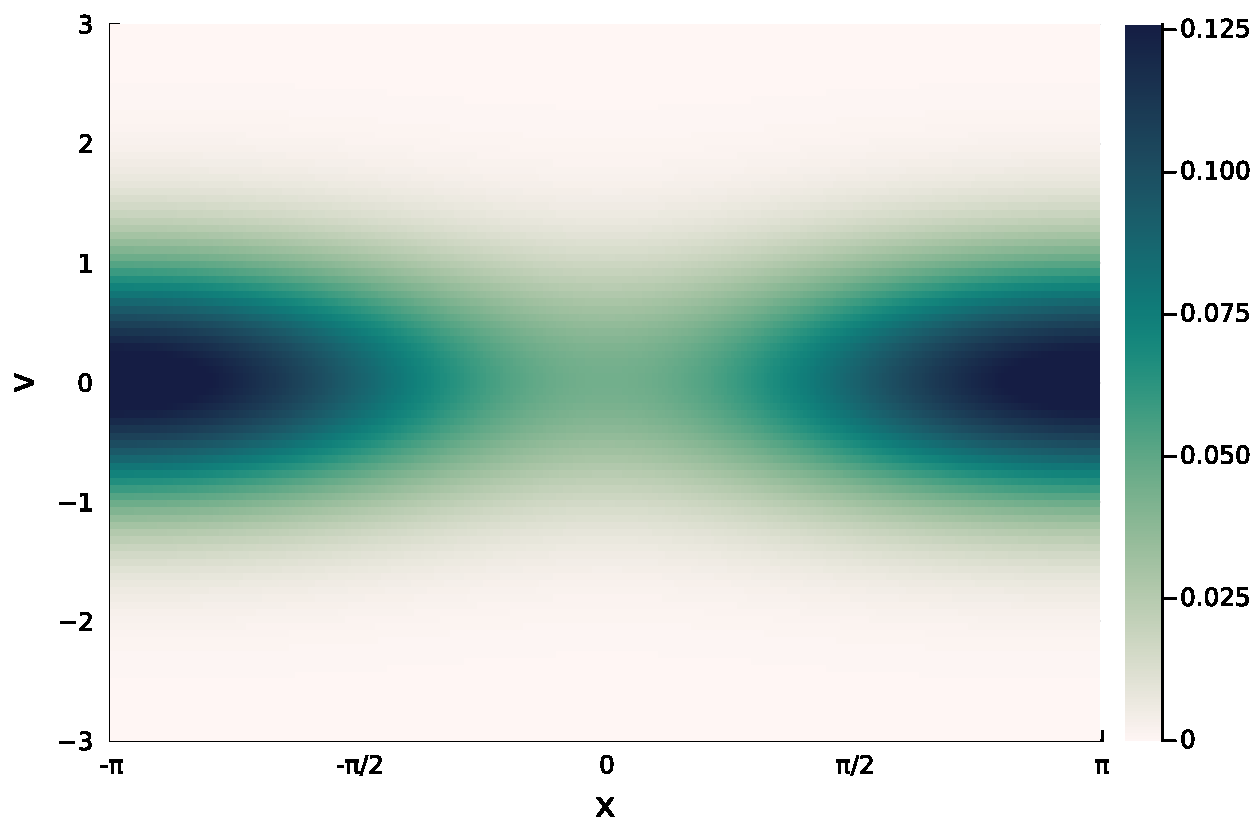
\includegraphics[width=\textwidth]{e_density_landau_t_0.pdf}
    \end{subfigure}
    \begin{subfigure}{0.45\textwidth}
        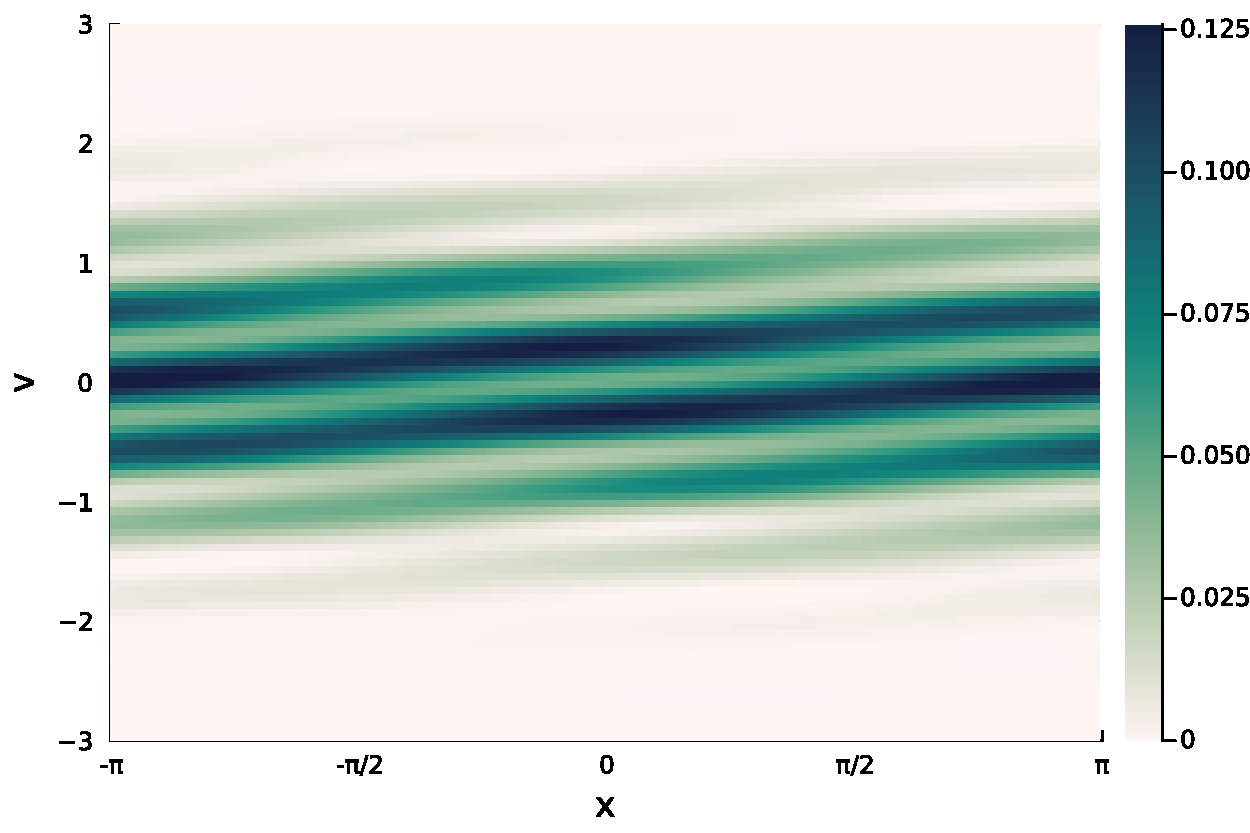
\includegraphics[width=\textwidth]{e_density_landau_t_10.pdf}
    \end{subfigure}
    \begin{subfigure}{0.45\textwidth}
        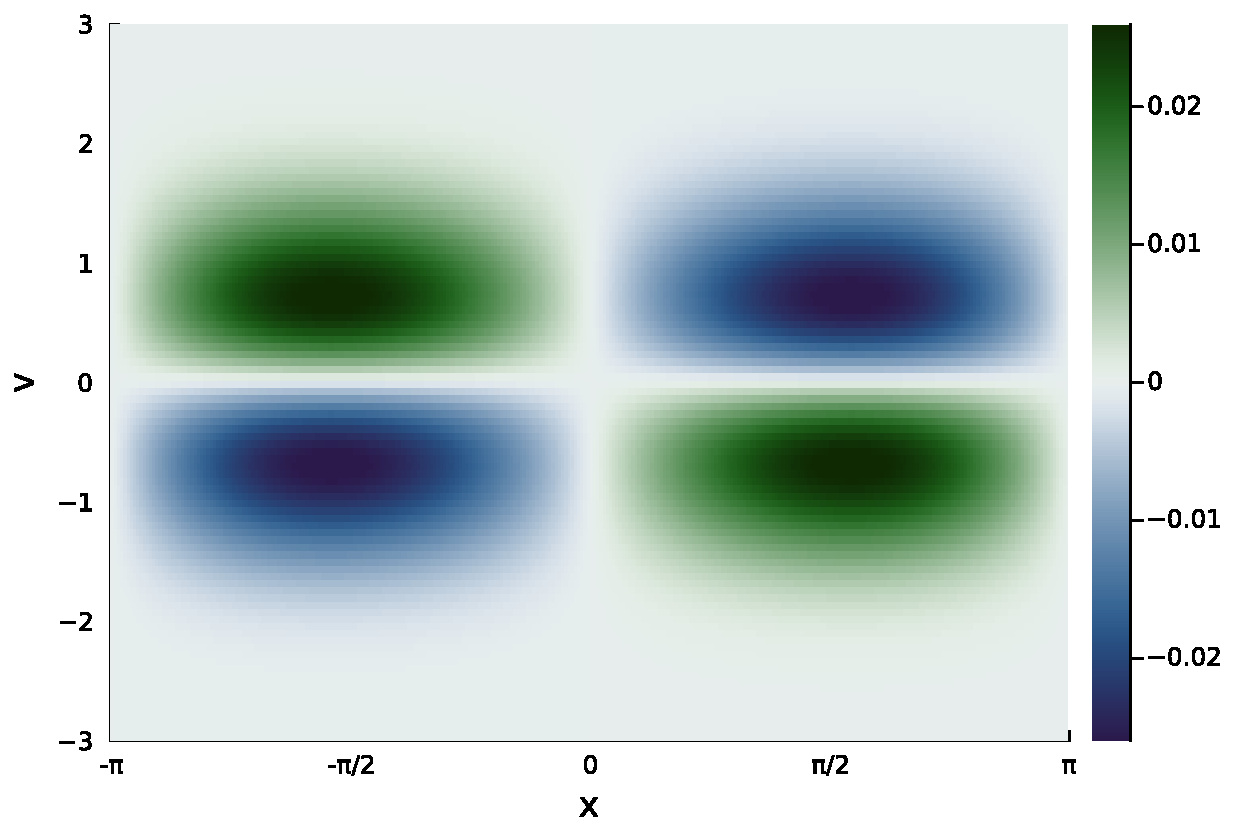
\includegraphics[width=\textwidth]{rhs_landau_t_0.pdf}
    \end{subfigure}
    \begin{subfigure}{0.45\textwidth}
        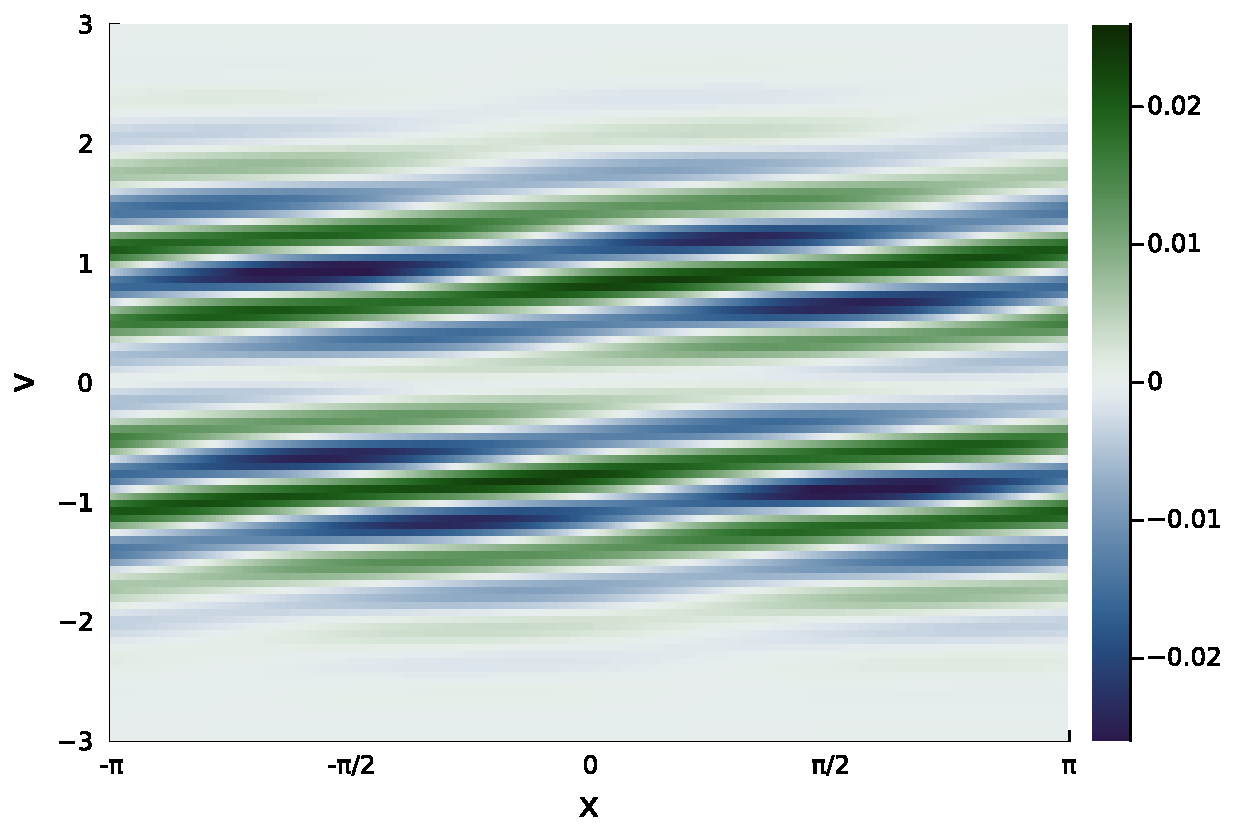
\includegraphics[width=\textwidth]{rhs_landau_t_10.pdf}
    \end{subfigure}
    \caption{
        Landau damping. 
        Top: $e^-$ density in $\Omega_x \times \Omega_v$. 
        Bottom: $RHS(f)$ for $f$ on top. 
        Left: Time $t = 0$. 
        Right: Time $t = 10$. 
    }\label{fig:density}
\end{figure}

\begin{figure}
    \centering
    \begin{subfigure}{0.45\textwidth}
        \missingfigure{$0$th moment (mass) for $m = 1, 2, 3, 5$}
    \end{subfigure}
    \begin{subfigure}{0.45\textwidth}
        \missingfigure{$1$st moment (momentum) for $m = 1, 2, 3, 5$}
    \end{subfigure}
    \begin{subfigure}{0.45\textwidth}
        \missingfigure{$2$nd moment (kinetic energy) for $m = 1, 2, 3, 5$}
    \end{subfigure}
    \begin{subfigure}{0.45\textwidth}
        \missingfigure{$5$th moment for $m = 1, 2, 3, 5$}
    \end{subfigure}
    \caption{
        Error in the continuity equations for the Landau damping scenario with 
        $\alpha = 10^{-3}$. 
    }\label{fig:moments_linear_landau}
\end{figure}

\begin{figure}
    \centering
    \begin{subfigure}{0.45\textwidth}
        \missingfigure{$0$th moment (mass) for $m = 1, 2, 3, 5$}
    \end{subfigure}
    \begin{subfigure}{0.45\textwidth}
        \missingfigure{$1$st moment (momentum) for $m = 1, 2, 3, 5$}
    \end{subfigure}
    \begin{subfigure}{0.45\textwidth}
        \missingfigure{$2$nd moment (kinetic energy) for $m = 1, 2, 3, 5$}
    \end{subfigure}
    \begin{subfigure}{0.45\textwidth}
        \missingfigure{$5$th moment for $m = 1, 2, 3, 5$}
    \end{subfigure}
    \caption{
        Error in the continuity equations for the Landau damping scenario with 
        $\alpha = 1/2$. 
    }\label{fig:moments_nonlinear_landau}
\end{figure}

\subsection{Two-stream Instability}\label{sec:two_stream}

The initial conditions in the Landau damping case can often show positive results 
due to the high amount of symmetry in the system. For this reason, we consider a 
nonsymmetric two-stream instabilility 

\begin{equation}
    f(x, v, 0) = \frac{1}{4 \pi} (1 + \alpha \cos(x)) \exp (-(v - \bar{v}/2)^2)
        + \frac{1}{4 \pi} (1 + \beta \sin(x)) \exp (-(v + \bar{v}/2)^2)
    %f(x, v, 0) = (1 + \alpha \cos (x)) \left( \exp(-(v - \bar{v})^2) + \exp(-(v + \bar{v})^2) \right) 
\end{equation}

for $\bar{v} \in \bbR$ and $\alpha, \beta \in \left[ 0, 1/2 \right]$, chosen
such that $f(0)$ is strictly positive. We use the same grid points, rank, and
time step as in the previous section. We note the translated gaussians can be
expanded as

\begin{equation}
    \exp(-(v - \bar{v}/2)^2) = \exp(-v^2) 
    \sum_{k \geq 0} \frac{\exp(-\bar{v}^2) \bar{v}^k}{2^k k!} H_k (v)
\end{equation}

where $H_k$ is the $k$-th Hermite polynomial. 

\begin{figure}
    \centering
    \begin{subfigure}{0.45\textwidth}
        \missingfigure{$e^-$ density for $t = 0$}
    \end{subfigure}
    \begin{subfigure}{0.45\textwidth}
        \missingfigure{$e^-$ density for $t = 10$}
    \end{subfigure}
    \caption{
        Two-stream instability. density for various times. 
    }\label{fig:density_two_stream}
\end{figure}

\begin{figure}
    \centering
    \begin{subfigure}{0.45\textwidth}
        \missingfigure{$0$th moment (mass) for $m = 1, 2, 3, 5$}
    \end{subfigure}
    \begin{subfigure}{0.45\textwidth}
        \missingfigure{$1$st moment (momentum) for $m = 1, 2, 3, 5$}
    \end{subfigure}
    \begin{subfigure}{0.45\textwidth}
        \missingfigure{$2$nd moment (kinetic energy) for $m = 1, 2, 3, 5$}
    \end{subfigure}
    \begin{subfigure}{0.45\textwidth}
        \missingfigure{$5$th moment for $m = 1, 2, 3, 5$}
    \end{subfigure}
    \caption{
        Error in the continuity equations for the two-stream instability. 
    }\label{fig:moments_two_stream}
\end{figure}

\iffalse
\begin{enumerate}
    \item Basic takeaway of Landau damping: dissipation can occur without loss of energy; 
          different than in fluid equations
    \item Specific initial conditions that we consider: 
          \begin{equation}\label{eq:initial_conditions}
            f (x, v, 0) = ( 1 + \alpha \cos (x) ) \exp (- v^2)
          \end{equation}
          for the parameter value $\alpha = 1/2$ computed over the domain 
          $\Omega_x = [ -\pi, \pi )_{per}$, $\Omega_v = [ -5, 5 ]$. $f$ is normalized 
          to have initial mass $1$. 
    \item This is too large of a parameter value to use linear approx from Landau's 
          original argument, but the derivation can be done to higher order and 
          dissipation is still analytically predicted. Indeed, we see this numerically as 
          well, see fig. \ref{fig:density}. 
    \item Odd power moments seem to have very predictable behavior. The error follows a 
          power/exponential law very well (see fig. \ref{fig:moments}). This must have something to 
          do with some form of symmetry wrt. $\Omega_v$. Are the kinetic moment density 
          functions 
          \begin{equation}
            \underbrace{v v \ldots v}_{k\text{ times}} f(x, v, t)
          \end{equation}
          symmetric wrt. $v$? All odd moments $\scrM_k$ are essentially $0$. Even power 
          moments seem more erratic but are lower long-term. This could be a power law, 
          though it is difficult to tell. Another, longer integration may be needed. 
    \item Observables seem to be near-constant whenever the density function is 
          positive, see fig. \ref{fig:positivity}. As soon as $f$ becomes negative, the 
          observables go haywire. Should a positivity-preserving method be considered? 
          How would this affect the conservation? 
\end{enumerate}
\fi

% -------------------------------------------------------------------------------------- %
